\subsection{Glyph: \glyph{Consumption}}
\label{sec:consumption}

\glyph{Consumption} is the arc used to represent the fact that an entity pool is consumed by a process, but is not produced by the process.

\begin{glyphDescription}

\glyphSboTerm
SBO:0000394 ! consumption

\glyphOrigin
One \glyph{EPN} (\sect{EPNs}).

\glyphTarget
One \glyph{process node} (\sect{PNs}).

\glyphSymbol
No particular symbol is used to represent a \glyph{consumption}, as shown in \fig{consumption}.

\end{glyphDescription}

\begin{figure}[H]
  \centering
  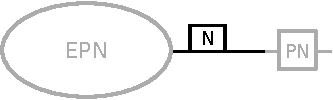
\includegraphics{images/build/consumption.pdf}
  \caption{The \PD glyph for \glyph{consumption}.}
  \label{fig:consumption}
\end{figure}

A cardinality label may be associated with \glyph{consumption} (\sect{consumption}) or \glyph{production} (\sect{production}) arcs, indicating the stoichiometry of a process.
This label is a number enclosed in a rectangular container with one of the long sides adjacent to the \glyph{consumption} arc.
The cardinality is required to eliminate ambiguity when the exact composition, or the number of copies, of the inputs or outputs to a reaction are ambiguous from the map.
An example is a multimer of six subunits dissociating into two monomers and two dimers.
Without stoichiometry labels another result, such as four monomers and one dimer could be inferred.
Once assigned to one arc connecting to a process node, cardinality should be represented on all \glyph{consumption} and \glyph{production} arcs connected to that process node to avoid misinterpretation.

Omitted cardinality on one edge only should not be treated as cardinality of one, but as an unspecified cardinality.
In most cases, the exact value may be derived from the context, but unless cardinality is explicitly shown, it should be considered as unspecified.
In the case where the stoichiometry of some part of the process is not known, or undefined, a question mark ("?") should be used within the cardinality label of the corresponding arcs.

% The following is for [X]Emacs users.  Please leave in place.
% Local Variables:
% TeX-master: "../sbgn_PD-level1"
% End:
